
\chapter{ROB Stall and Load Dependents}\label{ROB}\label{Chapter3:Recording ROB delay and ROB dependencies}
In this chapter, we discuss how, at run time, we keep track of the ROB head stall and the number of dependents of a load that stalls the ROB head and blocks instruction retirement.

\section{ROB Stall}
ROB stall is the  time for which an incomplete load instruction waits at the ROB head to complete~\cite{Superscalar}. In out-of-order-issue processors, multiple instructions run in parallel, but their results are committed in-order. The ROB is used for this purpose. It is a FIFO queue which maintains the order of instructions. An ``uncommitted'' result can, however, be used by any other in-flight instruction that depends on that result.
ROB head is a pointer which is used to commit instructions in order. So, if there is a load instruction at the ROB head waiting for getting data from memory, the subsequent instructions cannot be committed. If the ROB is full, no more new instruction can be added to the ROB.
So, the time for which an instruction waits at the ROB head to be committed is critical for performance and we will refer to it as critical delay.

\section{Dependent Instructions}
There are instructions which have a very high number of dependent instructions either in the execution pipeline or in the ROB. Such instructions are more critical for performance because they can stall the execution of many upcoming instructions. Therefore, the count of dependent instructions is an important metric for criticality along with the the ROB stall.

\section{Computing ROB Delay and Dependencies at Run-time}\label{ROB}
For calculating the ROB delay, we  first initialize the delay to the current cycle of the simulation when an instruction is put into the ROB. Then at the time of retirement or commit from the ROB, we take the difference from the current core cycle. This is not exactly the ROB head stall, but easier to compute and a reasonable measure to identify instructions that stay in the ROB for too long. We calculate this delay for only those
instructions that have at least one source operand or are load instructions.
To calculate instruction dependency count for a load instruction stalled at the ROB head, we maintain the dependence tree rooted at each load instruction~(the dependence tree of a load is a subtree of the bigger in-flight tree).

Our experimental results of ROB head stall are presented in the first two pages of Figure~\ref{fig:robstats}~(spread over the next five pages). While we collected the results for a large number of dynamic instruction traces of the SPEC CPU 2017 applications, for brevity we only show the results for selected traces of three applications, namely mcf, lbm and xalancbmk. The results are shown for three different configurations, namely without a prefetcher~(no) and with two different prefetchers i.e., SPP at the L2 cache and IPCP~(instruction pointer classifier-based prefetching)~\cite{IPCP} at the L1 cache. Since 90\% of load instructions have ROB head stall of one cycle, we exclude these loads from these statistics. The distribution of the remaining 10\% loads is shown in these bar charts. We show the percentage of these 10\% loads on the y-axis and collect statistics for a certain maximum ROB head stall. For example, the heights of the bars at the value of 20 cycles show the percentage of these loads that have ROB head stall in (10, 20] cycles. We see that most of these 10\% loads have ROB head stall in the range of (10, 20] cycles. For IPCP, the percentage of loads in the smaller ROB head stall bins is higher than SPP indicating that IPCP can hide load miss latency better. This is because of two reasons. First, IPCP is an inherently better prefetcher. Second, IPCP sits alongside the L1 data cache prefetching into the L1 data cache and as a result, is better equipped to hide load miss latency.

The last three pages of Figure~\ref{fig:robstats} show the distribution of the 10\% loads based on the number of dependents. We use the IPCP for collecting these statistics, although the number of in-flight dependents of a load depends only the compiled binary and the instruction window (or ROB) size. These statistics are shown for the dynamic instruction traces of three applications, namely gcc, cactuBSSN, and x264.
 \begin{figure}[h!]
 \caption{Experimental results for ROB delay and dependency (spread over the next six pages)}
 \label{fig:robstats}
 \end{figure}

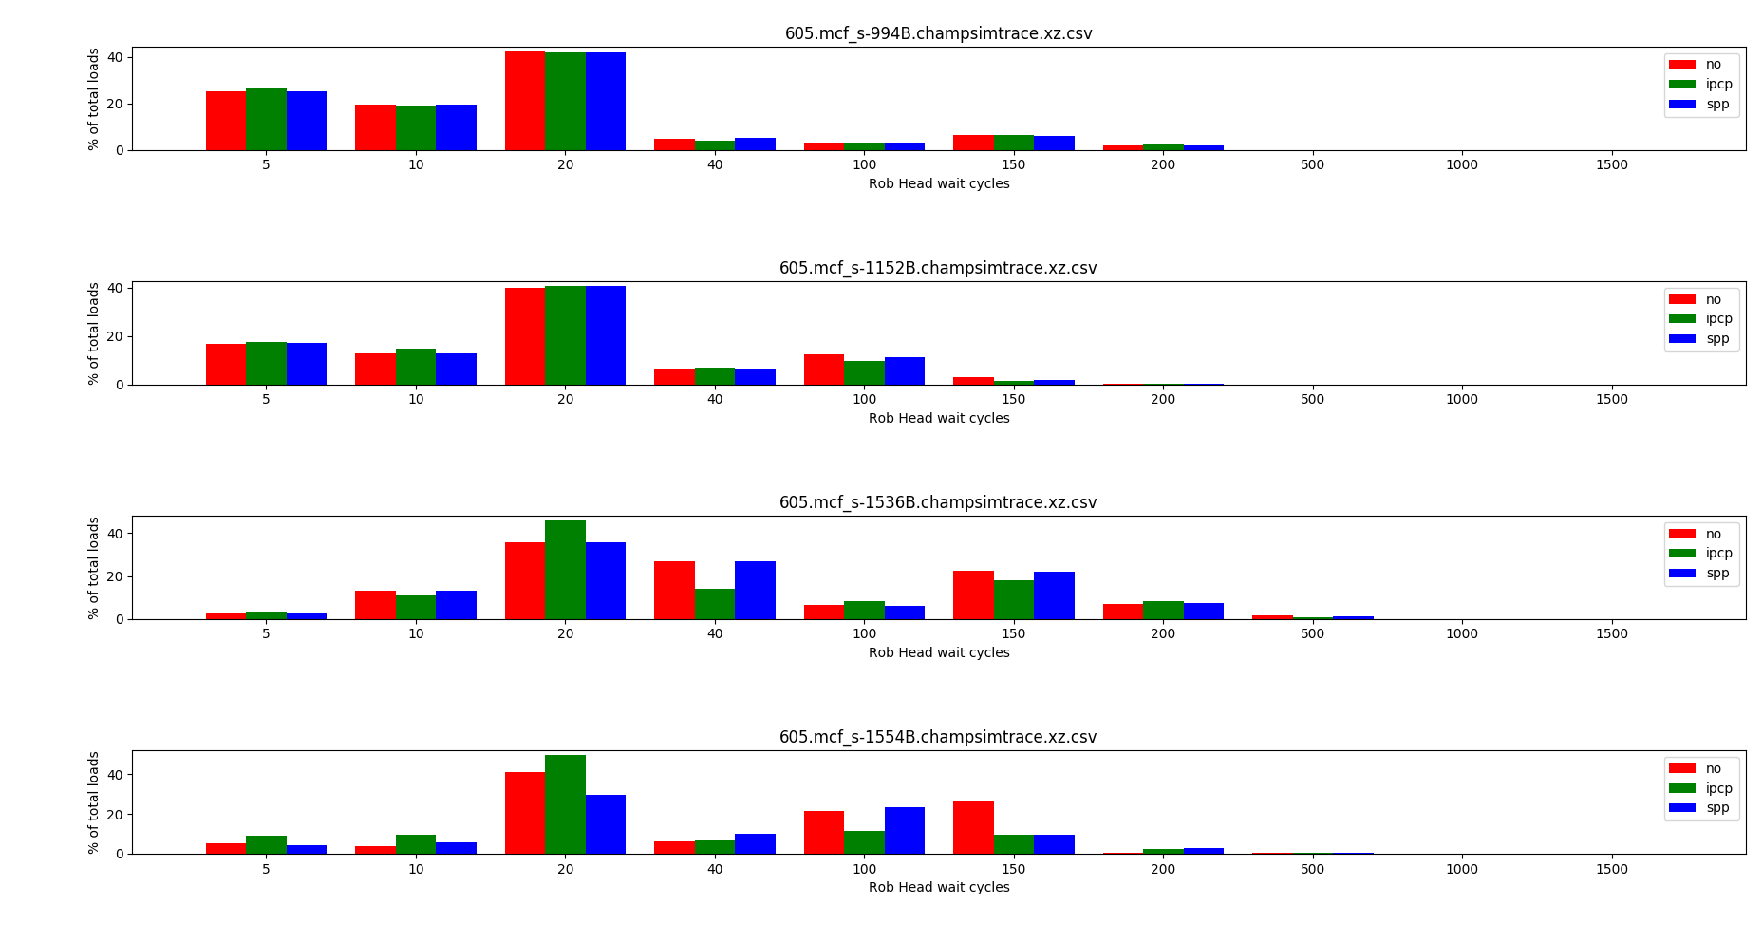
\includepdf[pages={1-} ]{images/rob.pdf}
\textbf{Our observations from Figure~\ref{fig:robstats} are summarized below.}
\begin{itemize}
\item Most of the instruction traces show ROB head stall up to  200 cycles. Some of the traces experience ROB head stall up to 500 cycles. 619.lbm\_s shows ROB head stall up to 1000 cycles.
\item Most of the loads from all the workloads show a dependence count of less than five.
\item Most of the loads in all traces show ROB head stall in the range of (10, 20] cycles.
\item There are some workloads which do not experience any improvement in ROB head stall cycles from any of the prefetchers.
\end{itemize}

\section{Storage of Critical IPs}

For keeping track of the critical load IPs and using them for prefetching, we store the IPs of the critical load instructions at run-time in a table  of predefined size. The table is fully-associative and exercises LRU replacement.
The table size is one of the parameters needed to be fine-tuned and we have empirically fixed it to 200 entries. Note that the physical implementation of this table can have four to eight banks each having 25-50 entries so that associative search latency of all banks in parallel can be kept within a reasonable limit. Note that we store only the IP of a critical load instruction and not the data addresses it touches.
Not storing the data addresses helps reduce the size of the table.
The interface of the critical IP table is shown in Figure~\ref{fig:criticaliptable}.
\begin{figure}[H]
{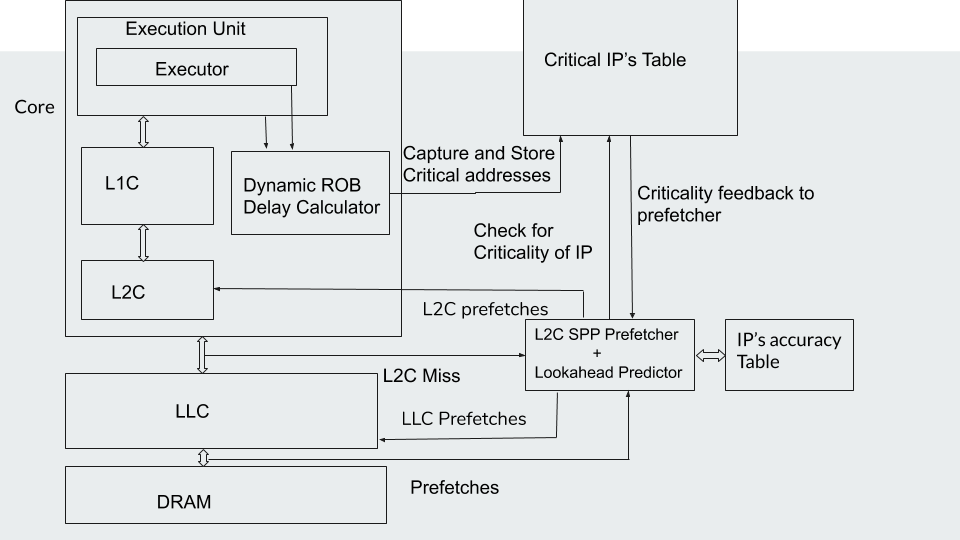
\includegraphics[scale=0.4]{images/Block.png}}\par\medskip
\caption{Structures to capture and use critical load IPs in a typical CPU}
\label{fig:criticaliptable}
\end{figure}

Once we have a table of the critical IPs, we can use this to tune prefetching. Generally, prefetchers get triggered for every miss address. So, by using this table as history of critical IPs, we can decide for any miss address sourced by a particular load IP, whether to prefetch or not or give more importance to this IP.

There are many ways to use critical IPs for tuning prefetching decision. For example, we can trigger prefetches for every miss address sourced by only the critical IPs or use criticality information alongside SPP offering a higher lookahead depth for the critical IPs. This thesis specifically focuses on using only critical IPs for prefetching and designing lookahead mechanisms for critical loads with all other structures same as in SPP. This allows us to squarely concentrate on how to use the criticality information in prefetching without worrying about computation of delta values, or maintaining signature tables, etc.. Our primary contributions toward effective computation of
lookahead depth of SPP given the set of critical IPs are discussed in the next chapter.

\section{Determining Critical IPs}\label{Crritical IP}
We use a combination of ROB head stall and dependence count of load instructions for deciding criticality and entry into the critical IP table. We use thresholds on ROB head stall and dependence count to decide which load instruction IPs are entered into the critical IP table.
The ROB head stall varies widely across applications and across loads of a single application. This makes it very difficult to have a meaningful static threshold for ROB head stall that works for all scenarios. In fact, we found that with static thresholds, we end up
having excessive prefetching for some of the applications, while some of the applications have almost no prefetching at all. Both ways, it is detrimental for performance. In general, the range of critical ROB head stall varies widely across applications and across different phases of the same application. Therefore, 
a mechanism is required that can dynamically adjust the critical ROB stall threshold depending on the current phase of the program and the trace.

We design an algorithm which dynamically adjusts the threshold depending upon the current behaviour of the program. We divide the range of ROB head stall in multiple bins e.g., (1, 10], (10, 20], etc. and count the frequency of each bin.
We also divide program execution into intervals where the interval length is predefined in terms of the number of critical loads. At the end of an interval, we use the frequencies of the ROB head stall bins to decide the ROB head stall threshold for the next interval and reset the frequencies. Specifically, 
we compute the sum of the frequencies of all the bins and start accumulating the frequencies starting from the highest stall bin to the lowest. We stop when the ratio of the cumulative frequency to the total frequency is at least a predefined coverage fraction. The ROB head stall bin where we stop defines the dynamic ROB stall threshold for the next interval to decide entry into the critical IP table.
The idea behind this algorithm is to have the minimal portion of the loads as critical loads that have the ROB head stall on the higher side. We empirically find that taking the top~(by ROB head stall) 1/4th to 1/7th fraction of the all loads as critical is effective. As we decrease this fraction, we start getting less number of critical addresses for prefetching and that helps decrease memory bandwidth consumption. We initialize the critial ROB head stall threshold to zero. This is found to be quite effective in having a healthy coverage to begin with, although this can put very high pressure on the cache and DRAM bandwidth in the initial learning phase.

Contrary to the variability in ROB head stall, the number of dependents of loads does not show a wide range of values. We empirically set a static threshold value of five on the dependent count.